\documentclass[]{article}
\usepackage{hyperref}
\usepackage{graphicx}
\usepackage{float}
\hypersetup{
	colorlinks=true,
	linkcolor=blue,
	filecolor=magenta,      
	urlcolor=cyan,
	pdftitle={Overleaf Example},
	pdfpagemode=FullScreen,
}
\newcommand{\quotes}[1]{``#1''}
%opening
\title{%
	Movies visual analytic tool \\
	\large Visual Analytics final project}

\author{Luca Giovannesi}
\date{}
\begin{document}

\maketitle

\section{Introduction}
IMDB is a website in which all moves data are collected, but, there isn't a built-in visual tool to analyzed these data, to analyze the data we have to open multiple pages and comparing data manually, this is inefficiently for large analysis, so i decided to develop a tool capable to do this kind of analysis, in particular with the main use cases for this software could be:
\begin{itemize}
	\item To discover new movies based by some criteria
	\item To discover new movies or similar to movies that you had already seen and you had like.
	\item To find trends, insights and curiosities on a large dataset of movies
\end{itemize}
\section{Related work}
During the development of the project, i thought of possible analysis cases in order to have a clear idea on what features are needed, so i started to search for reports or facts about the movie industries.\newline
The first idea in which the tool could be useful is to study the decline or the ascent of some genre and if possible to understand the reasons. I focused my attention on the western movies, since nowadays is very rare to have this genre at the cinema. There are a lot of article about this decline, i found the article \quotes{\emph{\href{https://screenculturejournal.com/2017/04/the-decline-in-popularity-of-the-western-film-genre/}{The Decline in Popularity of the Western Film Genre}}} written by \emph{Ben Pivoz} in which the author analyze the decline of the western genre.\newline\newline
One interesting analysis that could be performed in the movies industries, is if there is a correlation between the budget and the success of a movie, this was analyzed in the paper \href{https://asistdl.onlinelibrary.wiley.com/doi/full/10.1002/asi.23213}{\quotes{Correlations between user voting data, budget, and box office for films in the internet movie database}}, this paper other than trying to answer to this question, suggest to me also some features to implements, like taking in consideration the inflation, phenomenon completely ignored at the beginning of this project, furthermore the authors of this paper based their work on the IMDB dataset, the same dataset used in this project.
\section{Dataset}
\subsection{The used dataset}
The used dataset is the one called \quotes{\href{https://www.kaggle.com/datasets/rounakbanik/the-movies-dataset}{The Movies Dataset}} available on \href{https://www.kaggle.com/}{Kaggle}, this dataset contains about 5000 movies from the 1917 until 2017.\newline
The dataset is composed by 7 csv files, but the tool uses only 3 of them:
\begin{itemize}
	\item \textbf{\quotes{movie\_metadata.csv}}: This file has 24 columns and it contains the main information of the movies.
	\item \textbf{\quotes{keywords.csv}}: This file includes the keywords of each movies.
	\item \textbf{\quotes{credits.csv}}: This file contains information about the people who worked on the movies. 
\end{itemize}
\subsection{Dataset processing}
The dataset needs a data elaboration to create a new dataset customized for our tool, in this way the perform heavy computation are avoided in \quotes{realtime} in the visualization tool and the useless data are dropped in order to have a small dataset with a quicker loading time.\newline
Furthermore i take in consideration also the inflation, 1\$ of 1930s is not equivalent to 1\$ of nowadays, applying some calculation in this phase.\newline
This pre-processing phase is made by a python script and it is composed by 2 main phases:
\begin{enumerate}
	\item In this phase all the data from the different files are merged and the movies which contains invalid data, like empty fields or invalid formats, are dropped.
	\item The budget and revenue of each movie are computed also considering the inflation.
	\item This step computes the needed information for the multidimensional reduction, it is subdivided in 2 sub-phases:
	\begin{enumerate}
		\item \textbf{Build of similarity matrix}\newline
		A similarity matrix is build in which each cell $ij$ is filled with the similarity between the keywords of the movies $i$ and $j$
		\item \textbf{MultiDimensional Scaling positions}\newline
		Starting from the similarity matrix the position of each movie in the multidimensional scaling plot is computed.
	\end{enumerate}
\end{enumerate}
After the previous elaboration each movie has these fields:
\begin{itemize}
	\item \textbf{id}: An integer used to identify the movies.
	\item \textbf{Title}: The original title of the movies.
	\item \textbf{Genres}: The genres of the movies.
	\item \textbf{Release year}: The release year of the movies.
	\item \textbf{Runtime}: The runtime in minutes.
	\item \textbf{Spoken languages}: The spoken languages of the movies.
	\item \textbf{Vote avg}: The average of the votes.
	\item \textbf{Vote count}: The amount of the votes.
	\item \textbf{Revenue}: The revenue in dollars.
	\item \textbf{Revenue (Inf.)}: The actual revenue considering the inflation.
	\item \textbf{Popularity}: A popularity decimal value assigned by IMDB.
	\item \textbf{Budget}: The budget in dollars.
	\item \textbf{Budget (Inf.)}: The actual budget in dollars considering the inflation.
	\item \textbf{Keywords}:The keywords of each movies, they are not directly used by the tool, but they can be useful to understand if the MDS works well.
	\item \textbf{MDS position}: The coordinates of each movie in the MDS plot.
	\item \textbf{Director}: The movie's director.
\end{itemize}
So there are 16 fields and 4943 movies, this makes the AS index equal to $79088$ definitely bigger than the suggested one, so i have created also the option to filter the dataset taking only the top 1000 movies by popularity, with this smaller dataset the AS index is of $1600$ giving a smoother user interaction, especially on low-end PC.\newline
\section{Visualization Techniques}
\subsection{Main interface}
The tool include a short header with the project name and an option to select the two type of dataset, can be selected the full dataset with about 5000 movies or the smaller one with only the top 1000 movies by popularity.\newline
Since the dataset has a dimension of about 5 MB, the loading of the page can take some time if the user has a slow internet connection, so there is also a nice interface shown in the loading phase.
\subsection{Multidimensional scaling}
\begin{figure}[H]
	\centering
	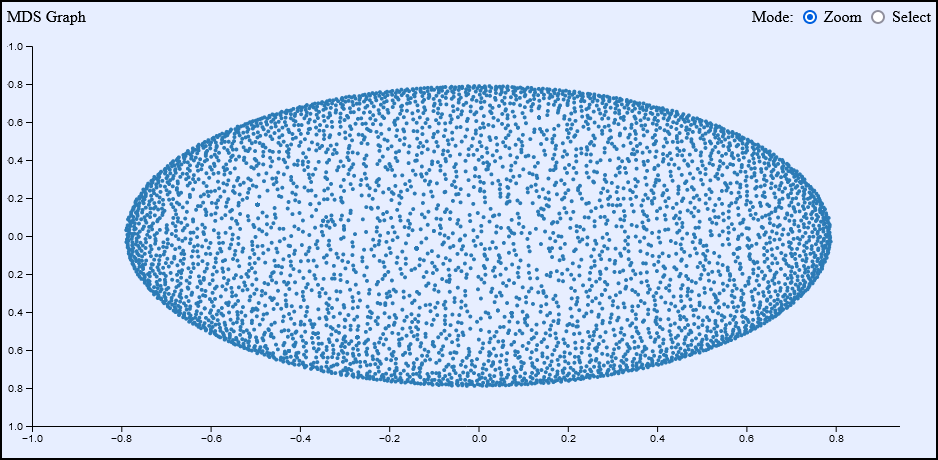
\includegraphics[width=1\linewidth]{images/mds_plot}
	\caption{Multidimensional plot}
	\label{fig:mdsplot}
\end{figure}
\subsubsection{Pre-Processing phase}
Multi-dimension scaling is a technique to show graphically the similarity between a set of elements, starting from a similarity matrix in which we have an item for each row and column, we can use an appropriate algorithm to set a position of the element in a N-dimensions space, in our case into a 2D space.\newline
In this project the similarity between the keywords of each movies is computed using the Jaccard distance, the Jaccard distance is defined as $J(A,B)=\frac{|A\cap B|}{|A\cup B|}$, initially i have tried to use the cosine similarity but the results was bad, while with the Jaccard distance the outcomes are definitely better.\newline
Each movie has a set of keywords, each keyword has also an associated id, so for each movie is easy to get a vector with all the associated ids of the keywords, from these vector of integers we can apply the Jaccard distance to get the similarity between the set of keywords.\newline
Once the similarity matrix was built, i have used the \emph{sklearn.MDS} function with parameters \emph{max\_iter=1000, dissimilarity="precomputed", n\_init=8, eps=1e-6}, to compute the position in the 2D plane for each movie.\newline
The described computations are not done in real time by the webpage, because they are processes heavy to compute and the computation take a lot of time, so they are done previously with a python script in order to have inside the dataset directly the data helpful to draw this graph.
\subsubsection{Visualization tool}
In the graph there are a set of dots, each dots represents a movie, the user can hover the mouse on a dot to see addition information (Movie title, Director and release year) and to highlight the movie on the other plots.\newline
The visualization tool has two modes: the zoom mode and the select mode, with the zoom mode the user can zoom and scroll the visualized area of the graph, while in select mode the user can select an area drawing a rectangle.
\subsection{Parallel coordinates}
\begin{figure}[H]
	\centering
	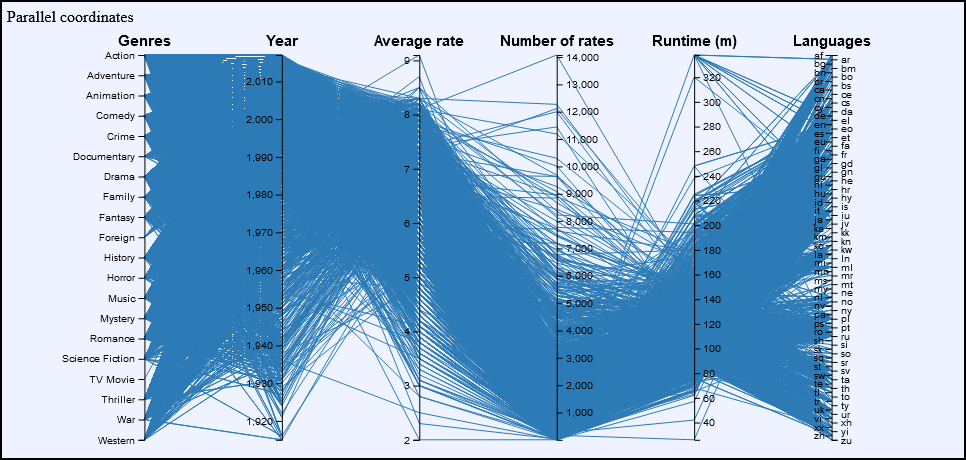
\includegraphics[width=1\linewidth]{images/parallel_plot}
	\caption{Parallel coordinates plot}
	\label{fig:parallelplot}
\end{figure}
Parallel coordinates is a technique uses to visualize multidimensional data through parallel axes in a 2D chart. In our case each axis represent an attribute of the movie.\newline
The visualized attributes are: genres, release year, average rate, number of rates, runtime and the spoken languages.\newline
The user can highlight a movie or makes a selection brushing a range selection on each axis.
\subsection{Bubble plot}
\begin{figure}[H]
	\centering
	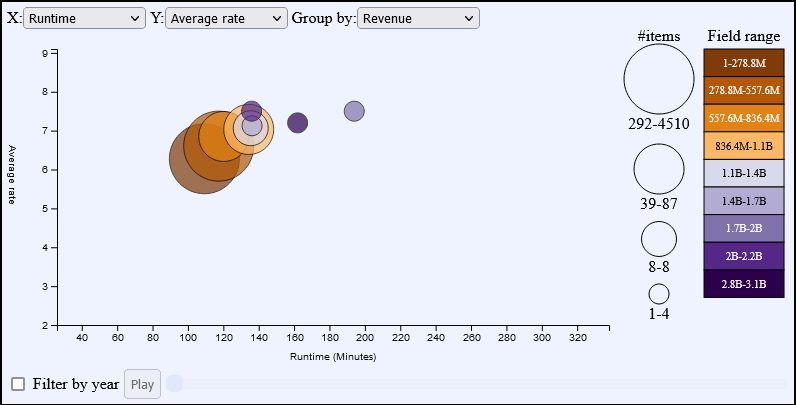
\includegraphics[width=1\linewidth]{images/bubble_plot}
	\caption[Bubble plot]{An instance of bubble plot with aggregation enabled.}
	\label{fig:bubbleplot}
\end{figure}
In the bubble plot we can visualize every continuous attribute present in the dataset, the user can select the attribute for the axes X and Y, he can also aggregate by a specific field, when the aggregation is enabled each bubble has a specific radius and color, the radius indicates the amount of elements inside the bubble, and the color the range of the selected field inside the bubble.
For example in the plot shown in the figure \ref{fig:bubbleplot} each bubble has the center in a point when the X position indicates the runtime and the Y position the average rate, the elements are grouped by the revenue, so for example the dark brown bubble represents the movies with a revenue between 1 million and 278.8 millions and it contains an amount of movies between 292 and 4510.\newline
The chosen colors are picked using \href{https://colorbrewer2.or}{ColorBrew2} and they are colorblind safe.\newline
In this graph is also possible to visualize only the movies of a specific year using the bottom slider, it is also possible to automatically go forward with the years clicking the button \quotes{play}.
\subsection{Column plot}
\begin{figure}
	\centering
	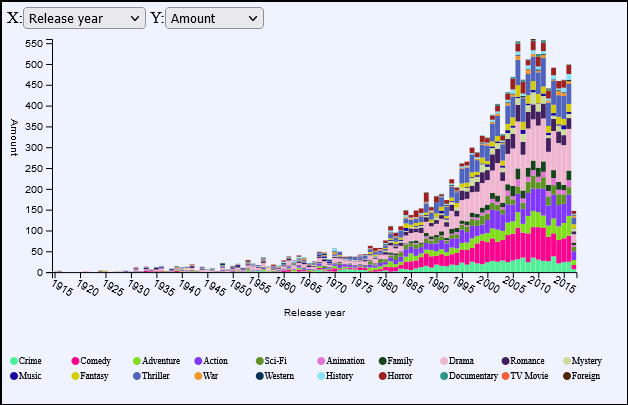
\includegraphics[width=0.49\linewidth]{images/column_plot}
	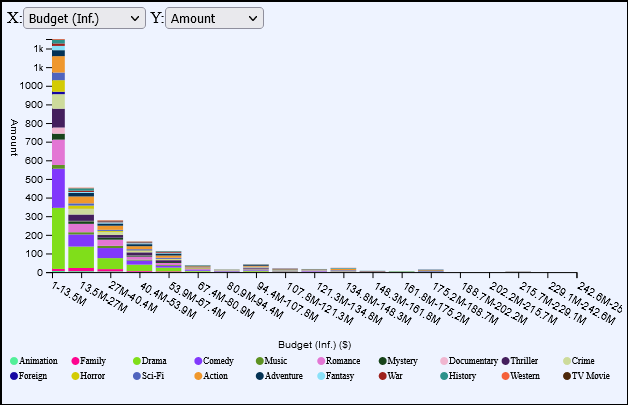
\includegraphics[width=0.49\linewidth]{images/column_plot1}
	\caption{Example of column plot visualization, on the left all the values of the X axis are visualized, while on the right are grouped in intervals.}
	\label{fig:columnplot}
\end{figure}
A column plot is build with a series of parallel columns to the axis X, the height of each column represents the value of the Y axis, in our case the amount of elements or the percentage ratio.\newline
Each column contains multiple segments of different colors, each color represents the genre of a movie and if for example a movie genre is both action and adventure, the movie will be counted twice.\newline
It is possible to choose different fields for the X axis, the user can choose between: release year, runtime, average rate, number of rates, revenue, revenue with inflation, popularity, budget and budget with inflation, while for the Y axis the user can choose between the amount of movies present in the X field or how the different genre are divided in percentage, for example in left image in figure \ref{fig:columnplot} we have the amount of movie release for each year divided by genre, but for example in the last years the amount of released movies is much larger than the ones released in 60', so can be useful to visualized the percentage of each genre during the years, this can be done selecting percentage on the Y axis, we will see this application in the insights.\newline
There are some fields in which all the possible values can be displayed, for example the years like in the left image in figure \ref{fig:columnplot}, while there are other fields that are impossible to represents all the value, for example the budget (right image of figure \ref{fig:columnplot}), so the column represent an aggregated value, for instance the first column represents the movies with a budget between 1 millions and 15 millions, the second from 15M and 30M and so on.\newline The user zoom on a specific area drawing a rectangle with the mouse, if the user zoom on an area composed by aggregated value, if there is enough space, the graph disable the aggregation and show the value singularly, otherwise the aggregation is still present.\newline\newline
At the bottom there is the legend with the colors associated at each movie, clicking on a genre is possible to filter the graph in order to visualize only the selected genre.
\subsection{Selection list}
\begin{figure}[H]
	\centering
	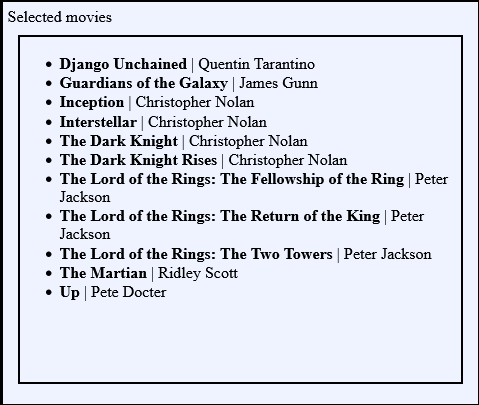
\includegraphics[width=0.7\linewidth]{images/selection_list}
	\caption[Selection list]{List of selected movies}
	\label{fig:selectionlist}
\end{figure}
When a selection is made, the list of the selected movies is displayed in the bottom right area, the list is in alphabetical order and shown the title of the movie and director name.
\subsection{Interaction}
\begin{figure}[H]
	\centering
	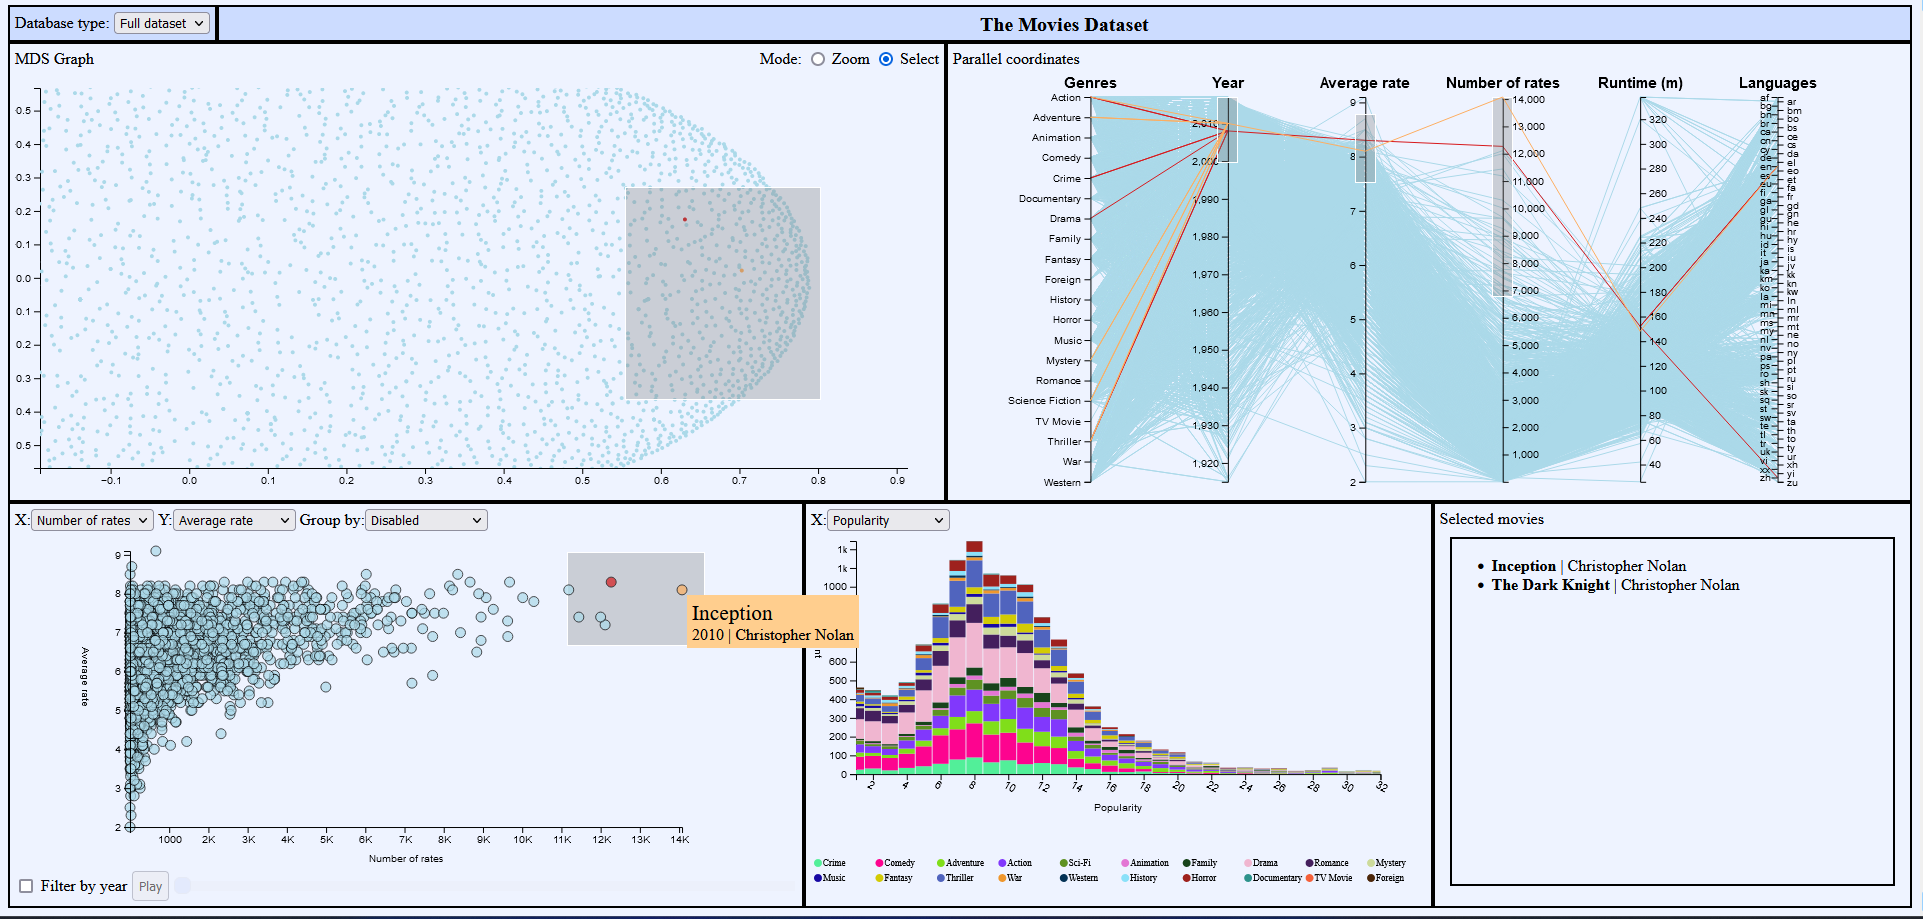
\includegraphics[width=1\linewidth]{images/interaction1}
	\caption[Interaction example]{An example of selection using multiple graph}
	\label{fig:interaction1}
\end{figure}
Each interaction on a graph triggers some events also in the other graphs, the implemented interaction regarding the selection are:
\begin{itemize}
	\item \textbf{Mouse hover:} When the mouse is hover an element, this item is colored by yellow in all the graphs. Furthermore a popup to show some information of the movie is shown.
	\item \textbf{Selection:} When the user select some elements on a graph, the selected elements are highlighted also on the other graphs. If the user makes a selection on multiple graph, the highlighted elements are the common movies between the selection of the different graphs.
\end{itemize}
\section{Insights}
\subsection{The decline of western movies}
The western genre had the maximum popularity between the the 1940s and 1970s, as mentioned in the article \href{https://screenculturejournal.com/2017/04/the-decline-in-popularity-of-the-western-film-genre/}{\quotes{The Decline in Popularity of the Western Film Genre}} \quotes{\emph{[...] For a long time, the Western was one of the dominant genres in the American film industry. After getting off to a good start in the silent film era, it declined throughout the 1920s and 30s before experiencing a resurgence in the 1940s. At that point, it became extremely popular in the United States [...]. However, beginning in the 1970s, audience appetite for the genre began to wane.[...]}}.
We expect to see a first decline between 1920s and 30s and an increase of popularity between 1940s and 70s.
\begin{figure}[H]
	\centering
	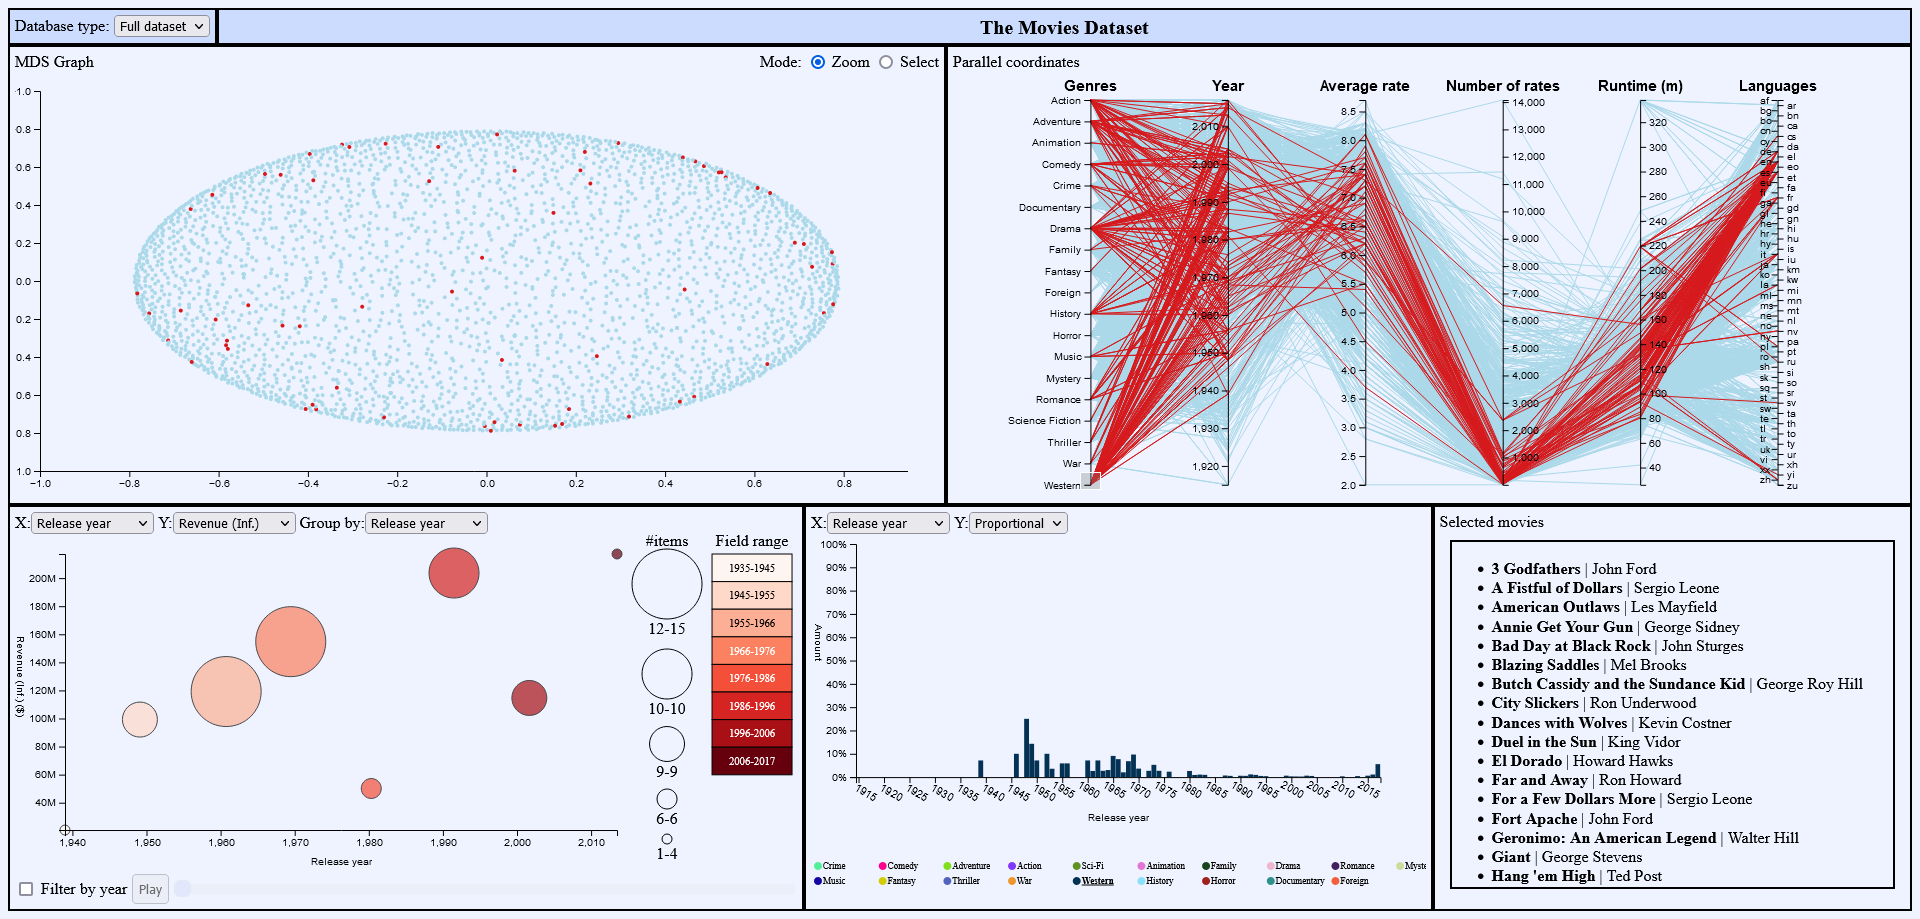
\includegraphics[width=1\linewidth]{images/insights_western}
	\caption[Western movies trend]{Analyis of the western movies among the years}
	\label{fig:insightswestern}
\end{figure}
In the instance presented in figure \ref{fig:insightswestern} we have on the column plot with X axis set to release years, in the Y axis the amount in percentage and we have filtered only the western movies. Unfortunately we can see the first decline between 1920s and 30s because these movies are not in the dataset, but, we can see the increase of popularity between 1945 until the 1975s, we can see also that starting from the 1980s the percentage of western movies is very small compared to the other genres, so we can see clearly the decline.\newline\newline
Using the parallel coordinates graph we have selected only the western movies, and setting the bubble plot with X for release year, revenue considering the inflation for Y and group the movies by the release year, we can make two observations in the bubble plot: 
\begin{enumerate}
	\item The amount of movies are smaller as the years increase (the dots get always smaller and smaller as you go to the right), this confirm the trend of the column plot.
	\item We can see how the western movies released between 60s and 70s have an higher revenue than the ones in 2000s, probably at that time the people were more interested to watch them.
\end{enumerate} 
\subsubsection{A larger budget makes a better movie?}
Spend a lot of money to produce a movie, ensure us to produce a better movie? This could be a popular question at which in the paper \quotes{\emph{Correlations Between User Voting Data, Budget, and Box Office for Films in the Internet Movie Database}} the autors have tried to get a response, and they conclude that \quotes{\emph{[...] we find a strong correlation between number of user votes and the economic statistics, particularly budget [...]}}
\begin{figure}[H]
	\centering
	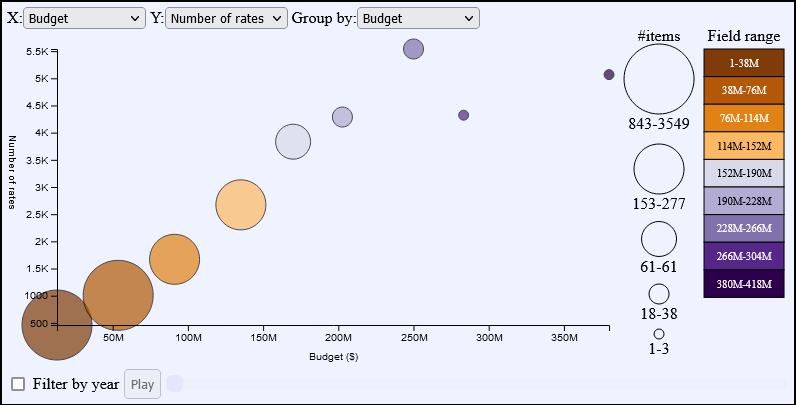
\includegraphics[width=1\linewidth]{images/insigth_budget}
	\caption{The usege of bubble plot to see the correlation between the budget and the number of rates}
	\label{fig:insigthbudget}
\end{figure}
Using the bubble plot we have set budget in the X axis, number of rates in Y axis, and the movies are grouped by budget, we can see that the number of rates increase as the budget increase, so we get the same result of the referenced paper.\newline
Caring also about the inflation the result is more accentuated. 
\subsubsection{Movie suggestions}
\begin{figure}[H]
	\centering
	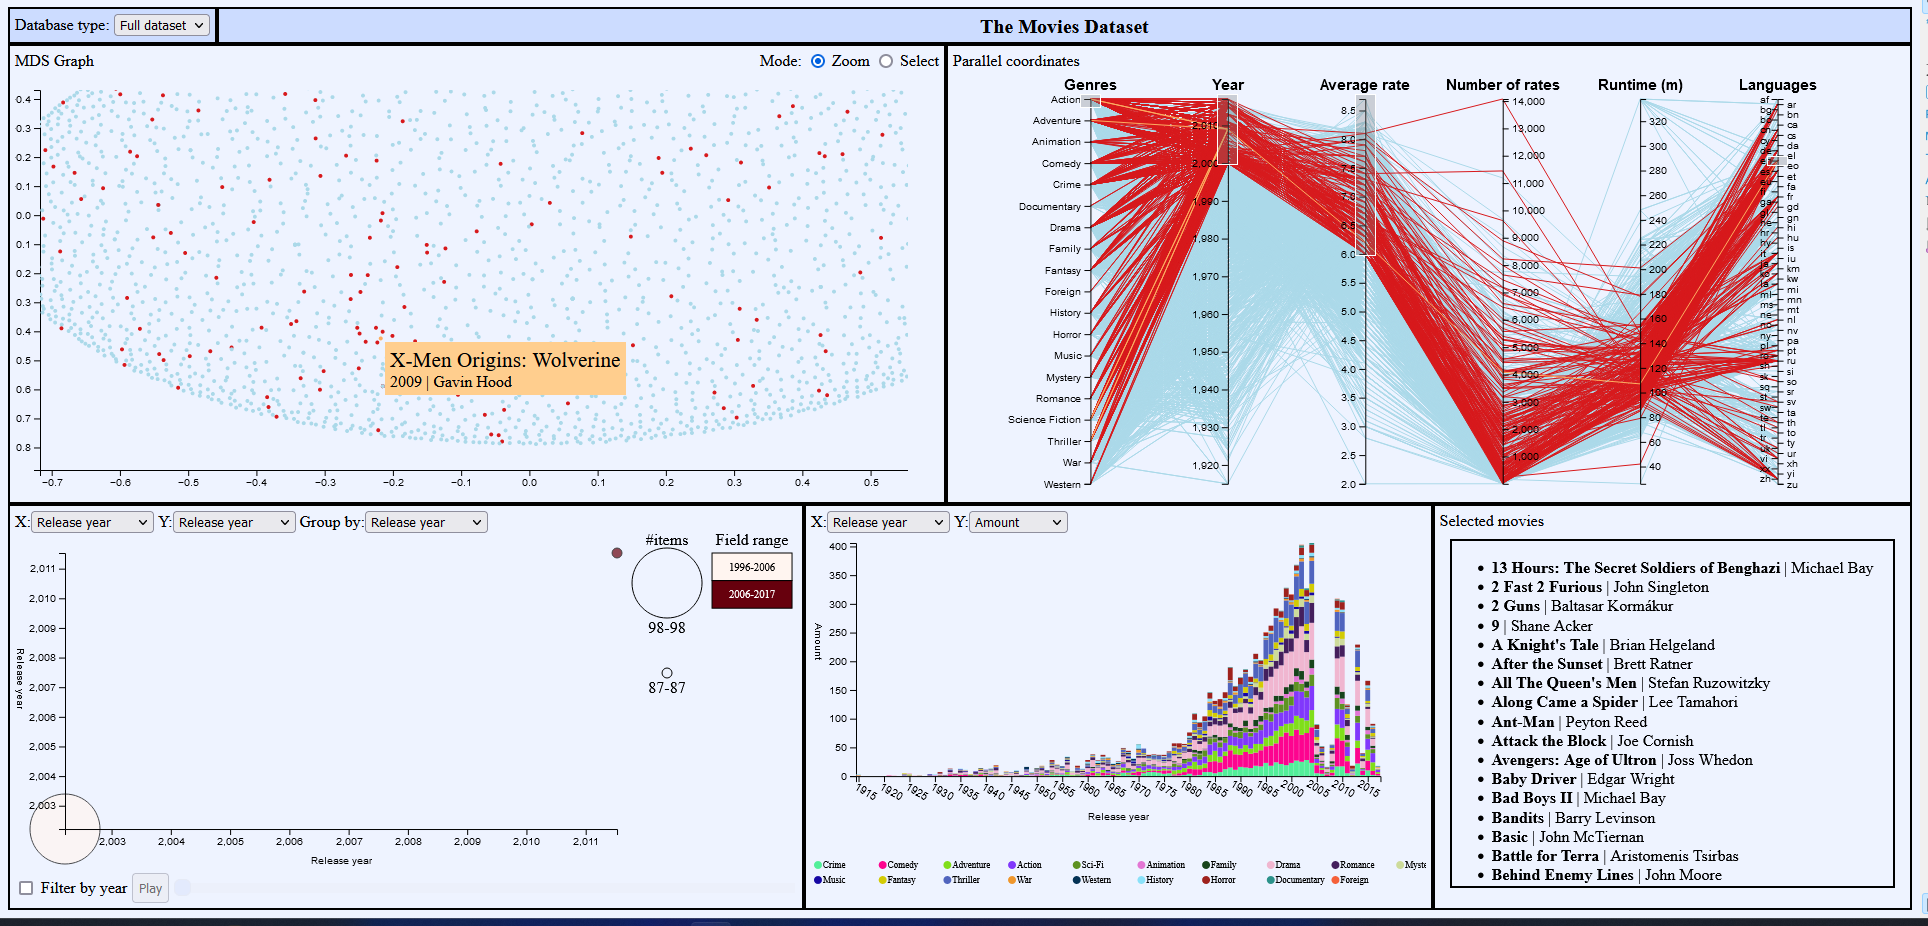
\includegraphics[width=1\linewidth]{images/insights_suggestion1}
	\caption{An instance in which the user search new movie based on the ones that he has already seen}
	\label{fig:insightssuggestion}
\end{figure}
\begin{figure}[H]
	\centering
	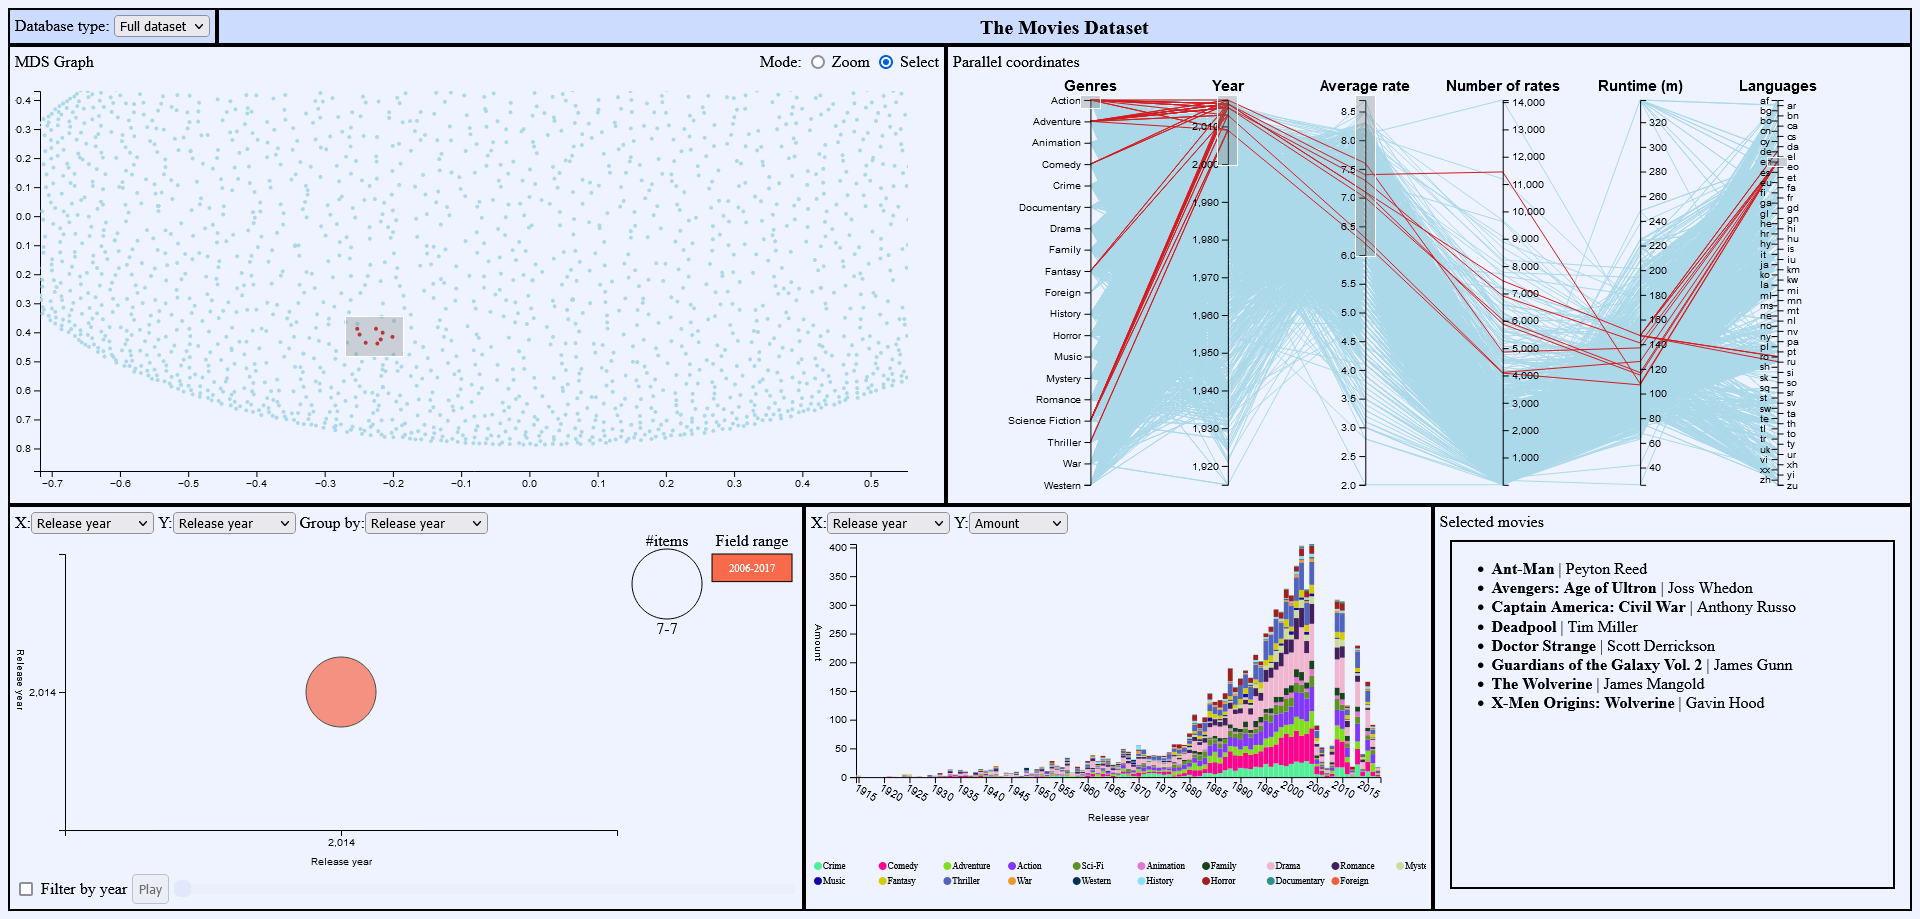
\includegraphics[width=1\linewidth]{images/insights_suggestion2}
	\caption{The user has selected the area find in figure \ref{fig:insightssuggestion} to have the list of movie on the right-bottom area}
	\label{fig:insightssuggestion2}
\end{figure}
With the MDS plot the user can find new movies based on the ones that he know, for example a user using the parallel coordinates can filter only the action movies, only the most recent ones (starting from 2000) and only the ones with a sufficient average score (to avoid to get bad movies as suggestions), now in the MDS plot only the movies that meet these criteria are highlighted by red (as shown in figure \ref{fig:insightssuggestion}), the user can move the mouse hover the highlighted elements to visualize the names until he get one movie that the user likes, for example the movie:\emph{Deadpool}.\newline
Once the user has find a movie that he like, he can switch the MDS plot to the selection mode to select the area near the found movie and he get the list of similar movies in the list located at bottom-right of the page.\newline
As we can see in figure \ref{fig:insightssuggestion2} the suggested movies are at most all with superheros so the multidimensional scaling on the similarity of the keywords works well.
\section{Conclusion}
The final version of the software allows to the users an interactive visual analytic of the cinema industry data, i am satisfied of the final result, every part works as expected, especially for the multidimensional part where i worked a lot and after multiple attempts it finally works almost fine, also if in future i will like improve this part because there are still some bad suggestions.
\end{document}
